\chapter{Servizio}
\label{chap:serv}
Preambolo
In questo capitolo verrá esposta l'architettura finale dell'applicativo sviluppato che permette la comunicazione tra il Surface Dial e la pagina web.\\
\section{Architettura Software}
Il progetto si presenta suddiviso in due parti ben distinte:
\begin{itemize}
\item \textbf{Servizio Angular}.
\item \textbf{Applicazione UWP} (Universal Windows Plaform).
\end{itemize}

\subsection{Servizio Angular}
In Angular, i Servizi rappresentano un tassello fondamentale per la realizzazione di un'applicazione. Un servizio è solitamente rappresentato da una classe indipendente dalla View che viene definita per svolgere un compito ben preciso ed effettuare delle operazioni strettamente correlate tenendo in mente il principio di singola responsabilità.\\
È possibile definire più servizi all'interno di un'applicazione, ognuno dei quali si occupa di portare a termine un determinato incarico incrementando la modularitá del progetto, inoltre un servizio puó a sua volta dipendere da altri servizi, che vengono definiti nel costruttore del servizio stesso.\\

Avvalendosi di Angular CLI, possiamo creare un Servizio tramite il comando:

\vspace{1.0cm}
\begin{lstlisting}[caption={Esempio creazione servizio},style=javaScriptCode]
	ng generate service <nome-del-servizio> <flag-opzionali>
\end{lstlisting} 
\vspace{1.0cm}
Una volta creati, i servizi possono essere iniettati all'interno di uno o più componenti grazie al meccanismo di \emph{Dependency Injection}.\\

Per poter utilizzare un servizio da noi definito, dobbiamo registrarlo con uno degli Injector presenti in Angular. Esiste infatti una gerarchia di Injector, che Angular provvede a creare, alla base dei quali c'è il cosiddetto Root Injector, che viene creato in fase di bootstrap dell’applicazione e i servizi registrati con quest’ultimo sono disponibili per tutta l’applicazione.\\

Per ogni Injector esiste sempre una sola istanza di un determinato servizio, come specificato nella documentazione ufficiale:\\

\emph{"Services are singletons within the scope of an injector. That is, there is at most one instance of a service in a given injector."}\\

L’ Injector si occupa di creare le dipendenze e si serve di un Provider, un oggetto il quale indica all'Injector come ottenere o creare un'istanza di una dipendenza.
Per ogni dipendenza che si vuole usare nell'applicazione si deve registrare un provider con un Injector, in modo che quest'ultimo possa poi utilizzare il provider per creare nuova istanza di quella dipendenza.

\subsubsection{Singleton services}

Per restare in linea con le direttive utilizzare dal gruppo Loccioni nello sviluppo dei loro servizi, abbiamo utilizzato il forRoot() pattern per l’injection del servizio nell’applicazione.\\

Questo pattern permette di specificare un modulo personalizzato per il servizio, il quale contiene un metodo statico chiamato appunto forRoot() che restituisce un ModuleWithProvider parametrizzato al modulo del Servizio.\\

Questo pattern permette di effettuare l’import del modulo nell’AppModule richiamando il metodo forRoot(), cosi da non dover appesantire il Provider del modulo iniziale e in linea di principio é bene utilizzarlo quando un provider prende in ingresso dei parametri, così da non dover specificarli ogni qualvolta il modulo venga utilizzato.

\subsubsection{DialService}

Lo scopo finale del servizio che abbiamo implementato é quello di poterlo utilizzare come ponte o intermediario tra il Surface Dial, che si interfaccia nativamente con l'applicazione UWP, la quale contiene una WebView con all'interno caricata una pagina custom Loccioni, e i componenti della View all'interno della pagina che intendono utilizzare il servizio.\\

Il componente che dipenderá da questo determinato servizio, chiamato appunto DialService, potrá facilmente utilizzare le funzionalitá messe a disposizione dal Surface Dial e interpretare gli eventi intercettati a RunTime.\\

Il core del servizio implementato è rappresentato dalla Classe DialService, essa infatti si occupa di inizializzare il servizio e rendere disponibile la comunicazione bi-direzionale tra il lato Web e quello UWP.In particolare si occupa di recuperare l'oggetto C\# iniettato a sua volta dentro l'oggetto window della pagina web, con visibilitá globale.\\

\vspace{1.0cm}
\begin{lstlisting}[caption={Recupero oggetto C\#},style=javaScriptCode]
	this.dial = (window as any).dial;
\end{lstlisting} 
\vspace{1.0cm}

L'oggetto dial viene poi inserito per questioni di sicurezza in una classe DialProxy, la quale implementa a sua volta l'interfaccia da noi sviluppata DialBackendBridge, nella quale sono presenti tutte le funzionalitá dell'oggetto "dial", richiamabili quindi da Web.

\subsubsection{DialProxy}

Al fine di aggiungere un livello di sicurezza sull’oggetto iniettato e sul suo successivo utilizzo, abbiamo deciso di implementare una classe chiamata DialProxy con la responsabilitá di wrappare l’oggetto e quindi di intercettare le chiamate fatte su di esso.\\

La classe DialProxy prende quindi in ingresso nel suo costruttore un oggetto di tipo DialBackendBridge, che rappresenta l'oggetto iniettato, e come secondo parametro il servizio DialService per poter accedere rapidamente alle proprietá del servizio e poter effettuare determinati controlli prima di richiamare un metodo.\\

\vspace{1.0cm}
\begin{lstlisting}[caption={Wrapping oggetto recuperato},style=javaScriptCode]
	this.dialProxy = new DialProxy(this.dial, this);
\end{lstlisting} 
\vspace{1.0cm}

\newpage
\subsubsection{DialBackendBridge}

DialBeckendBridge rappresenta l'interfaccia contenente la dichiarazione dei metodi implementati nella classe DialController dell'applicazione UWP.\\
In questo modo, tramite l'oggetto dial iniettato, sará possibile richiamare a RunTime i metodi dichiarati nel C\# attraverso il Web.\\

\vspace{1.0cm}
\begin{lstlisting}[caption={Interfaccia DialBackendBridge},style=javaScriptCode]
export interface DialBackednBridge{
		
	getProductId(): string;
	
	setMenu(arrayOfItem: any[]): void;
	
	clearMenu(): void;
	
	deleteItem(tag: string): void;
	
	addItem(item: any): void;
	
	createDialMenuItem(tag: string, displayText: string, icon: string): any;
	
	setDefaultItem(defaultItems: string[]): void;
	
	manualInvoke(tag: string): void;		

}		
\end{lstlisting} 
\vspace{1.0cm}

\newpage
\subsubsection{DialFrontendBridge}

Per rendere questa comunicazione bi-direzionale, abbiamo creato una classe DialFrontendBridge con la responsabilitá di rendere visibili dei metodi all'interno dell'oggetto window e quindi richiamabili tramite script dall'applicazione UWP.\\

L'invocazione di questi metodi comporta la successiva emissione di un determinato evento a coloro che vi si sottoscrivono, con la possibilitá del passaggio di parametri di tipo stringa.\\

Tramite l'utilizzo degli EventEmitter messi a disposizione dal core di Angular e definiti come mostrato nel codice sottostante, la classe DialFrontendBridge permette all'utilizzatore del servizio di sottoscriversi a determinati eventi pubblici, che quando richiamati emettono un determinato valore. RIFERIMENTO A CODICE \\

\vspace{1.0cm}
\begin{lstlisting}[caption={EventEmitter esposti da DialFrontendBridge},style=javaScriptCode]
public onRotationEvent = new EventEmitter<{tag: string, degree: string}>();
public onPressedRotationEvent = new EventEmitter<{tag: string, degree: string}>();
public onClickEvent = new EventEmitter<string>();
public onInvokeEvent = new EventEmitter<string>();
public onScreenContactStartedEvent = new EventEmitter<{x: string, y: string}>();
public onScreenContactContinuedEvent = new EventEmitter<{x: string, y: string}>();
public onScreenContactEndedEvent = new EventEmitter();
\end{lstlisting} 
\vspace{1.0cm}

Affinché questi metodi possano essere richiamati tramite script dall'applicazione UWP é stato necessario inserire l'istanza della classe all'interno dell'oggetto window, cosi da renderlo visibile e utilizzabile dall'esterno.\\

\vspace{1.0cm}
\begin{lstlisting}[caption={Inserimento classe DialFrontendbridge in window },style=javaScriptCode]
(windowa as any).DialFrontendBridge = this.dialFrontendbridge;
\end{lstlisting} 
\vspace{1.0cm}

\newpage
\vspace{1.0cm}
\begin{lstlisting}[caption={Metodi esposti da DialFrontendBridge},style=javaScriptCode]
   /**
     * Metodo richiamato da UWP che notifica la rotazione del Microsoft Dial.
     * @param tag Identificatore dell'elemento che ha eseguito la rotazione
     * @param degree Gradi della rotazione
     */
    public RotationEvent(tag: string, degree: string): string{
        this.onRotationEvent.emit({tag, degree});
        return degree;
    }

    /**
     * Metodo richiamato da UWP che notifica la rotazione de
     * l Microsoft Dial con il Dial premuto.
     * @param tag Identificatore dell'elemento che ha eseguito la rotazione
     * @param degree Gradi della rotazione
     */
    public PressedRotationEvent(tag: string, degree: string): string{
        this.onPressedRotationEvent.emit({tag, degree});
        return degree;
    }

    /**
     * Metodo richiamato dall'UWP che notifica la pressione del del Microsoft Dial.
     * @param tag Identificatore dell'elemeto che ha eseguito il click sul Dial.
     */
    public ClickEvent(tag: string){
            this.onClickEvent.emit(tag);
    }

    /**
     * Metodo richiamato dall'UWP che notifica l'invocazione di un elemento di Menu.
     * @param tag Identificatore del MenuItem che ha eseguito l'invoke.
     */
    public InvokeEvent(tag: string){
        this.onInvokeEvent.emit(tag);
    }

    /**
     * Metodo richiamato dall'UWP che notifica il contatto del 
     * dispositivo Dial con lo schermo nel punto con coordinate x e y.
     * @param x Coordinata x della posizione
     * @param y Coordinata y della posizione
     */
    public ScreenContactStartedEvent(x: string, y: string){
        this.onScreenContactStartedEvent.emit({x, y});
    }

    /**
     * Metodo richiamato dall'UWP che notifica lo spostamento del 
     * dispositivo Dial sullo schermo nel punto con coordinate x e y.
     * @param x Coordinata x della posizione
     * @param y Coordinata y della posizione
     */
    public ScreenContactContinuedEvent(x: string, y: string){
        this.onScreenContactContinuedEvent.emit({x, y});
    }

    /**
     * Metodo richiamato dall'UWP che norifica 
     * quando il Dial viene rimosso dallo schermo
     */
    public ScreenContactEndedEvent(){
        this.onScreenContactEndedEvent.emit();
    }
\end{lstlisting} 
\vspace{1.0cm}

\subsubsection{DialMenuLoader}

Il secondo servizio implementato, chiamato DialMenuLoader é un perfetto esempio di come usufruire del servizio DialService all'interno di Componenti o Servizi.\\

DialMenuLoader ha lo scopo di creare dinamicamente le voci di Menu da inserire nel dial e di definire per ciascuna voce il comportamento, che in questo caso rappresenta la navigazione tra le voci di menu di un ServerLayout Loccioni.\\

Grazie al servizio DialService e a quello Router inseriti nel costruttore, questo sotto-servizio permette di sottoscriversi automaticamente agli eventi di navigazione della pagina e a quelli del dial, così da caricare le giuste voci del menu in base al livello in cui si trova, caricando la voce di menu Home solo se si "atterra" in un componente altrimenti quella Back per navigare il menu nel senso opposto.\\

\begin{lstlisting}[caption={Metodo loadLevelMenuUp},style=javaScriptCode]
    /**
     * Carica un menu nel Dial e lo rende navigabile.
     * @param menu Menu da caricare nel Dial.
     */
    public loadMenu(menu: Menu){
      this.menu = menu;
      this.menuSubscribe();
      this.currentParent = this.menu.items[0];
      this.loadLevelMenuUp(this.currentParent);
    }
\end{lstlisting} 
\vspace{1.0cm}

Il servizio espone un metodo pubblico chiamato \textbf{loadMenu()}, il quale prende come parametro in ingresso un oggetto di tipo \emph{Menu} passatogli dal layout dell'applicazione contente tutte le voci di Menu disponibili all'interno della pagina web.\\

\begin{lstlisting}[caption={Metodo loadLevelMenuDown},style=javaScriptCode]
     /**
     * Carica i menu contenuti nell'item.
     * @param item Item su cui caricare i sotto-menu
     */
    private loadLevelMenuDown(item: MenuItem){
      this.currentMenuList = [];
      item.items.forEach(child => {
        this.currentMenuList.push(
          this.dialService.dialProxy.createDialMenuItem(
            child.containerId,
            child.label, 
            child.icon
            ),
          );
        },
      );
      this.currentMenuList.push(
        this.dialService.dialProxy.createDialMenuItem(
          'Back',
          'Back', 
          'back'
          ),
        );
      this.dialService.dialProxy.setMenu(
        this.currentMenuList
      )
    }
\end{lstlisting} 
\vspace{1.0cm}

Il metodo svolgerá le opportune analisi per ogni voce di menu contenuta e creerà dinamicamente le voci di menu da inserire nel menu del dial con i relativi comportamenti al richiamo di uno di essi, attraverso i metodi privati \textbf{loadLevelMenuDown()} e \textbf{loadLevelMenuDown()}.\\

\vspace{1.0cm}
\begin{lstlisting}[caption={Metodo loadLevelMenuUp},style=javaScriptCode]
    /**
     * Carica il livello di voci di menu sopra parent.
     * @param parent MenuItem contenente il livello corrente.
     */
    private loadLevelMenuUp(parent: MenuItem){
      this.currentMenuList = [];
      if (parent.level === 1){
        this.menu.items.forEach(item => {
          this.currentMenuList.push(
            this.dialService.dialProxy.createDialMenuItem(
              item.containerId, 
              item.label, 
              item.icon
            )
          );
        }
      );
      }else{
        this.menu.planItems.filter((value) => {
          return value.level === parent.level && value.parent === parent.parent;
        }).forEach((item) => {
          this.currentMenuList.push(
            this.dialService.dialProxy.createDialMenuItem(
              item.containerId, 
              item.label, 
              item.icon
            )
          );
        }
        );
        this.currentMenuList.push(
          this.dialService.dialProxy.createDialMenuItem(
            'Back', 
            'Back', 
            'back'
          )
        );
      }
      this.dialService.dialProxy.setMenu(this.currentMenuList);
    }
\end{lstlisting} 
\vspace{1.0cm}

Inoltré, attraverso i metodi \textbf{componentSubscribe()} e \textbf{menuSubscribe()} il servizio effettua dinamicamente le sottoscrizioni e disiscrizioni agli eventi interessati per la navigazione tra le voci di Menu.


\vspace{1.0cm}
\begin{lstlisting}[caption={Metodo componentSubscribe},style=javaScriptCode]
/**
* Sottoscrivzione avviata quando si atterra in un componente 
* da una voce di menu attraverso la navigazione con il dial
*/
private componentSubscribe() {
  this.dialService.flagForHome = true;
  this.dialService.dialProxy.setMenu([]);
  this.componentListener = 
  this.dialService.dialFrontendBridge.onInvokeEvent.subscribe(
   (tag: string) => {
     if (tag === 'home'){
	this.dialService.flagForHome = false;
	this.currentParent = new MenuItem();
	this.currentParent.level = 1;
	this.loadLevelMenuUp(this.currentParent);
	this.menuSubscribe();
	this.componentListener.unsubscribe();
	this.router.navigateByUrl('/server');
      }
    }
  );
}
\end{lstlisting} 
\vspace{1.0cm}

\vspace{1.0cm}
\begin{lstlisting}[caption={Metodo menuSubscribe},style=javaScriptCode]
/**
* Sottoscrizione avviata durate la nagivazione tra le voci di menu non leaf
*/
private menuSubscribe(){
	this.dialService.flagForHome = false;
	this.menuListener = 
	this.dialService.dialFrontendBridge.onInvokeEvent.subscribe(
	(tag: string) => {
	if (tag === 'Back'){
		this.loadLevelMenuUp(this.currentParent);
		this.currentParent = this.currentParent.parent;
		}else{
			this.menu.planItems.forEach(item => {
				if (tag === item.containerId){
					if (item.isLeaf){
						this.navigateToLeaf(item);
						this.menuListener.unsubscribe();
						this.componentSubscribe();
						this.currentParent = item;
					}
					else{
						this.loadLevelMenuDown(item);
						this.currentParent = item;
					}
				}
			});
			}
		}
	);
}

\end{lstlisting} 
\vspace{1.0cm}

\subsubsection{Widget}

Un widget Aulos è un componente in esecuzione all’interno di una DashBoard con lo scopo di rappresentare o modificare i dati ottenuti dal backend collegato fisicamente ad una macchina.\\

Nella nostra applicazione abbiamo modificato degli Widgets giá esistenti, utilizzando all'interno di essi il nostro servizio \emph{DialService}, allo scopo di renderli controllabili attraverso il Dial.Siamo partiti tentando di agganciarsi ad un semplice Widget che visualizza un range di possibili valori rappresentato da uno \emph{slider grafico}, con l'intento di variare, anche solo graficamente, il valore corrente attraverso l'evento rotazione del Dial.\\

\begin{lstlisting}[caption={Sottoscrizione evento rotazione Radial Gauge},style=javaScriptCode]
if (this.widget.runMode){
  if (this.dialService.isDialConnected){
	this.createMenuVoice();
	this.dialService.dialFrontendBridge.onRotationEvent.subscribe(
	({tag, degree}) => {
	  if (tag === this.id){
		this.value += (parseInt(degree, 10) * 5);
		this.changeDetectorRef.detectChanges();
	  }
	});
  }
}
\end{lstlisting} 


La stessa cosa è stata fatta per un widget rappresentato graficamente da un \emph{Radial Gauge}, fino ad arrivare a modificare valori lato Backend attraverso il DialChannelWidget, un widget creato da noi che contiene al suo interno , al contrario degli widget già presenti, il collegamento a \emph{N} diversi canali modificabili.
Questo ci ha permesso di sviluppare delle funzionalità custom per quel determinato Widget al fine di poterne acquisire il controllo, e scegliere canale per canale, il valore da settare, permettendo la variazione non solo grafica ma anche effettiva dei dati mostrati.\\

Per rendere sicura queste funzionalità abbiamo previsto la variazione dei valori con la singola rotazione e la successiva modifica lato backend qualora il dial venga premuto, altrimenti attraverso la funzionalità combinata di pressione e rotazione, così da evitare una involontaria modifica nel momento della presa possesso.\\

Analogamente all'evento sopra mostrato, chiamato onRotationEvent, gli eventi al quale il widget ChannelDialWidget si sottoscrive al fine di variare i valori di un canale selezionato, sia graficamente che in modo permanente lato backend, sono i seguenti:

\begin{itemize}
\item \textbf{onRotationEvent} 
\item \textbf{onClickEvent} 
\item \textbf{onPressedRotationEvent}
\end{itemize}

Durante la sua inizializzazione, il widget si sottoscrive all'evento di Invoke, con lo scopo di intercettare il tag sul quale viene richiamato il medesimo metodo dal Dial. Successivamente, se l'invoke richiamato restituisce il tag corrispondente all'ID del Widget in ascolto, viene pulito il menu del dial e vengono caricate le voci di menu inerenti ai canali collegati a quel determinato Widget cosi da poter essere richiamati e intercettati a loro volta dalla sottoscrizione all'evento onInvokeEvent.
 
\subsection{Applicazione UWP}

La seconda parte, invece, è costituita da un’ applicazione UWP ovvero Universal Windows Platform, presa in considerazione poiché la più recente tra i framework Microsoft e tra le sue caratteristiche troviamo la sicurezza e la portabilità tra le diverse piattaforme windows, ciò consente un maggiore supporto nel tempo e intercambiabilità tra i dispositivi dove utilizzarla.\\

L’applicazione DialBridge ha come responsabilità quella di comunicare con il Dispositivo HID attraverso le librerie fornite da Microsoft e allo stesso tempo comunicare con la pagina Web contenuta al suo interno.\\

Inizialmente abbiamo creato un’unica soluzione contenente sia la Web View che il Core dell’applicazione, ma abbiamo riscontrato un problema nell’injection dell’oggetto utilizzato per la comunicazione Web-UWP, poichè esso deve necessariamente essere iniettato a runtime.\\

Di conseguenza abbiamo creato due diverse soluzioni:

\begin{itemize}
\item \textbf{Core:} Contiene il nucleo dell’applicazione.
\item \textbf{EmbeddedBrowserView:} Contiene la parte runtime del progetto e effettua l’injection dell’oggetto nella pagina Web.
\end{itemize}

\subsubsection{Core}

Nel Core è contenuta la parte del progetto UWP che non richiede la partenza a runtime e comprende le seguenti classi:

\begin{itemize}
\item AulosCollection
\item AulosIcon
\item DialController
\item WebNotifier
\item DialMenuItem
\end{itemize}

\subsubsection{AulosCollection e AulosIcon}

Queste due classi si occupano, insieme al main, della parte riguardante le icone che verranno poi visualizzate nel menu del Dial. All’avvio dell’applicazione nella classe main viene effettuata una chiamata GET ad un eventuale server Loccioni che consente di ricevere un file JSON contenente una mappa “nome”-”FontGlyph” che verrà poi utilizzato per creare un DialMenuItem insieme al Font Aulos creato da Loccioni.\\

L’utilizzo di questo approccio consente una maggiore facilità nella sostituzione delle icone, che non dipende dalle risorse dell’applicazione stessa ma da un server Loccioni.

\subsubsection{DialController}

La classe DialController è una tra le più importanti poiché una sua istanza verrà poi inserita all’interno della WebView e servirà al servizio DialService per la comunicazione Web-UWP. I metodi pubblici al suo interno sono gli stessi dell’interfaccia DialBackendBridge che vengono utilizzati appunto tramite l’oggetto iniettato inizialmente.\\

Al suo interno troviamo un’ istanza della classe RadialController, ovvero la libreria Microsoft che permette la manipolazione del Dial, un'istanza di RadialControllerConfiguration e infine un notifier.\\

Nel costruttore abbiamo assegnato agli eventi presenti nella classe RadialController il relativo handler nella classe WebNotifier, in questo modo ogni volta che verrà emesso un determinato evento la pagina web riceverà una notifica e verrà svolta la funzione associata a quella determinata voce di menù.

\subsubsection{WebNotifier}

La classe WebNotifier contiene al suo interno una istanza della WebView ed ha come responsabilità quella di fornire i metodi che verranno poi utilizzati come EventHandler per gli eventi forniti dalla classe RadialController, in modo tale da riuscire a comunicare, attraverso la WebView al suo interno, alla pagina web l’emissione dell’evento stesso.\\

Al suo interno è presente anche un oggetto della classe CoreWindow utilizzato per spostare la posizione del mouse sullo schermo al primo contatto del Dial sulla superficie.

\subsubsection{DialMenuItem}

La classe DialMenuItem è una classe “modello” utilizzata per rappresentare un elemento contenuto nel Menu del Dial.

\subsubsection{MainPage}

Nella Main Page avviene l’inizializzazione dei componenti RadialController e la navigazione alla pagina web desiderata.\\

All’interno del metodo NavigationStarting troviamo il metodo AddWebAllowedObject che ci permette, una volta caricata la pagina, di iniettare l’oggetto della classe DialController per la comunicazione.

\section{Funzionalità implementate}

\subsection{Aquisizione widget}
\subsection{Posizionamento su schermo}

Uno dei maggiori vantaggi dell’utilizzo di un surface Dial è la possibilità di posizionarlo sopra uno schermo compatibile e di cambiare il suo funzionamento in base alla posizione utilizzata.
Questa funzionalità è gestita dal sistema operativo e comunica solamente con elementi nativi UWP, considerando ciò, abbiamo cercato un servizio Angular che ci permettesse di svolgere la stessa funzione all’interno di una pagina web ma senza risultati.
\begin{figure}[htpb!]
  \centering
  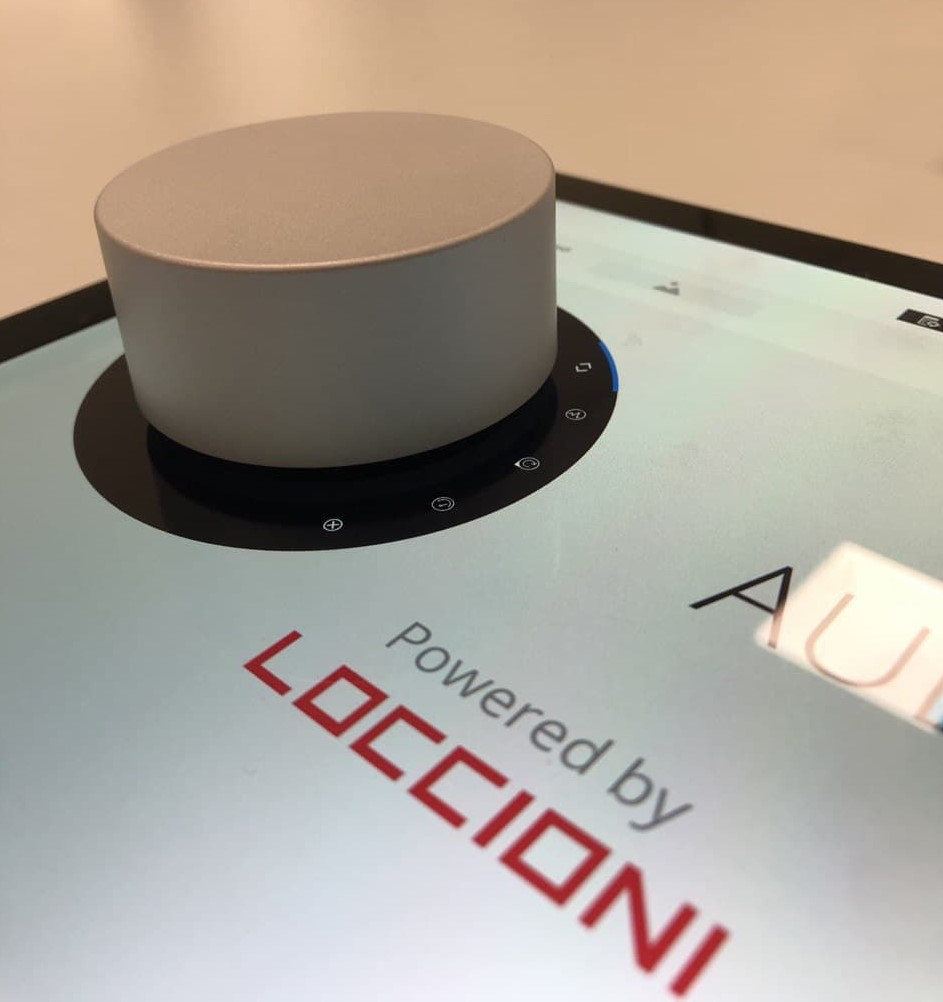
\includegraphics[width=0.5\textwidth]{DialSchermo}
  \caption{Microsoft Dial posizionato sopra un surface pro 6}
\end{figure}
Inizialmente abbiamo preso in considerazione la possibilitá di suddividere il layout dell’applicazione nativa in N riquadri, all’interno dei quali avremo posizionato il relativo Widget da controllare. Questa soluzione presenta peró delle limitazioni, in quanto in base alla risoluzione del dispositivo utilizzato, i widget caricabili in ogni riquadro del layout erano limitati al numero di riquadri definiti dall’applicazione UWP.

Abbiamo quindi cercato una soluzione, che spostasse la responsabilitá di acquisire il posizionamento lato Web anziché lato UWP. Dopo vari tentativi, abbiamo escogitato una soluzione che ci permettesse di avere un numero variabile di Widget configurabili nella Dashboard e la successiva acquisizione di essi, per fare ciò abbiamo sfruttato
Analizzando gli eventi richiamabili dalla classe RadialController, in particolare quelli inerenti al contatto con lo schermo, abbiamo notato prendevano in ingresso un oggetto di tipo RadialControllerScreenContact fornitogli dalla Libreria. Questo oggetto possiede due attributi relativi al Posizionamento ( Position ) e al Bound ( Bounds ) del rettangolo generato dal Dial sullo schermo.

Grazie all’attributo Position di tipo Point, é possibile ottenere, attraverso le coordinate X e Y, il punto centrale nel quale il Dial é posizionato.

\vspace{1.0cm}
\begin{lstlisting}[caption={Metodo ScreenContactStartedAsync},style=javaScriptCode]
 internal async Task ScreenContactStartedAsync(
 	RadialControllerScreenContactStartedEventArgs args
 )
  {
    this.simpleHaptics = args.SimpleHapticsController;
    string x = args.Contact.Position.X.ToString();
    string y = args.Contact.Position.Y.ToString();
    window.PointerPosition = new Point(
    	args.Contact.Position.X, 
    	args.Contact.Position.Y
    	);
    string function = 
    "window.DialFrontendBridge.ScreenContactStartedEvent('" + x + "', '" + y + "')";
    await webView.InvokeScriptAsync("eval", new string[] { function });
    onScreen = true;
    inputInjector.InjectMouseInput(new[] { inputInfo });
    inputInfo.MouseOptions = InjectedInputMouseOptions.Move;
    inputInfo.DeltaY = 1;
  }
\end{lstlisting} 
\vspace{1.0cm}


Attraverso la libreria Window.UI.Core é possibile spostare il cursore in un punto definito della UI corrente. Per questo motivo, la classe WebNotifier presente un attributo private e readonly chiamato window, un oggetto di tipo WindowCore che permette di intercettare eventi relativi ai dispositivi di Input utilizzati ma anche di posizionare il cursore del dispositivo in una posizione specifica in base alle coordinate passategli. In questo modo, attraverso l’attributo PointerPosition siamo stato in grado di creare un nuovo oggetto di tipo Point con le coordinate X e Y acquisite dal Dial consentendoci di posizionare il cursore in quel determinato punto.
\vspace{1.0cm}
\begin{lstlisting}[caption={Spostamento cursore},style=javaScriptCode]
  window.PointerPosition = new Point(args.Contact.Position.X, args.Contact.Position.Y);
\end{lstlisting} 
\vspace{1.0cm}
Questa soluzione ci ha permesso di spostare dinamicamente il cursore nella posizione centrale al disotto del Dial quando viene posizionato sopra lo schermo così da poter intercettare lato Web la posizione del cursore e permettere agli utilizzatori del servizio di riprodurre il comportamente appropriato per il Widget sopra il quale ci si posiziona.
Abbiamo quindi previsto nel Template HTML del Widget un metodo OnMouseOver che venisse richiamato solamente qualora il Dial fosse effettivamente a contatto con lo schermo, ma il semplice spostamento del cursore nella nuova posizione non richiamava correttamente il metodo in quanto il cursore non effettuava un movimento, ma veniva ricreato in quella determinata posizione.
Affinché la soluzione ideata funzionasse correttamente abbiamo importato una libreria chiamata Windows.UI.Input.Preview.Injection che mette a disposizione funziolitá per la simulazione di eventi di input.

Una volta posizionato il cursore nella nuova posizione, siamo stati in grado di simulare un impercettibile movimento del cursore di un singolo pixel, grazie al quale ci é stato possibile intercettare correttamente l’evento OnMouseMove dichiarato nel Template del Widget eseguendo il metodo associato.

\vspace{1.0cm}
\begin{lstlisting}[caption={Spostamento cursore},style=javaScriptCode]
inputInjector.InjectMouseInput(new[] { inputInfo });
inputInfo.MouseOptions = InjectedInputMouseOptions.Move;
inputInfo.DeltaY = 1;
\end{lstlisting} 
\vspace{1.0cm}
\subsection{Feedback aptico}
\subsection{Variazione degree personalizzata}
\section{Utilizzo del Servizio}

Per utilizzare il servizio DialService, occorre importarlo nel costruttore del componente che si sta sviluppando, in questo modo avremo accesso agli eventi che ci consentono di avere notifiche dal Dial.
Inizialmente è necessario creare una voce di Menù che rappresenta il widget all’interno del menù del Dial, così da avere la possibilità di acquisirne il controllo ed avere accesso alle sue funzionalità.
Sotto è riportato un esempio di creazione di una voce di menù per il dial con la relativa aggiunta alla lista di voci di Menu giá presenti.

\vspace{1.0cm}
\begin{lstlisting}[caption={Creazione nuova voce da widget},style=javaScriptCode]
  private createMenuVoice() {
    const dialMenuVoice = this.dialService.dialProxy.createDialMenuItem(
      this.widget.id, this.widget.descriptor.shortText, this.widget.descriptor.icon);
    this.dialService.dialProxy.addItem(dialMenuVoice);
  }
\end{lstlisting} 
\vspace{1.0cm}

Una volta aggiunta la voce di Menu al Dial, essa potrá essere selezionata attraverso il metodo Inkove messo a disposizione dalla classe DialController. Il metodo Invoke per acquisire una voce di menu, potrá essere richiamato sia attraverso il menu contestuale del Dial che compare nello schermo, che tramite un nostro metodo chiamato appunto ManualInvoke che esegue questa azione manualmente, richiamando tramite Web il medesimo metodo, solamente se quella voce di menu é presente tra quelle disponibile nel Dial.
In questo modo, il Widget non dovrá fare altro che mettersi in ascolto del metodo onInvokeEvent, il quale quando richiamato, restituisce una stringa definita “tag”, rappresentante la voce Menu acquisita.
Se quel tag, corrisponde all’id del Widget in ascolto, significa che l’utente ha richiesto il controllo di quel determinato Widget.

\vspace{1.0cm}
\begin{lstlisting}[caption={Ascolto Invoke della voce di menu'},style=javaScriptCode]
  this.dialService.dialFrontendBridge.onInvokeEvent.subscribe(tag => {
        if (tag === this.widget.id) {
          this.isActive = true;
          this.dialService.widget = this.widget.id;
          this.widgetDialStart();
          this.dialService.dialProxy.manualInvoke(this.channels[0].parameter.value);
        }
\end{lstlisting} 
\vspace{1.0cm}

Una volta acquisito il controllo del Widget, bisognerá mettersi in ascolto delle funzioni richiamabili dal Dial, attraverso gli eventEmitter messi a disposizione dalla classe DialFrontndBridge, e implementare il comportamento di quel Widget all’emissione di determinati eventi come la Rotazione o il Click.


\vspace{1.0cm}
\begin{lstlisting}[caption={Ascolto eventi associati alla voce di menu' selezionata},style=javaScriptCode]
const rotation = this.dialService.dialFrontendBridge.onRotationEvent.subscribe(
	({ tag, degree }) => {
      // Azione associata all'evento rotazione del Dial.
      if (tag === this.channels[this.currentChannel].parameter.value) {
        this.setSetterAtIndex(this.currentChannel, 
        parseNumber(degree)* this.moltiplicator
        );
      }
    });

const click = this.dialService.dialFrontendBridge.onClickEvent.subscribe(
	(tag) => {
      // Azione associata all'evento click del Dial.
      if(tag === this.channels[this.currentChannel].parameter.value){
          this.setChannelValue(this.channels[this.currentChannel].parameter.code,
          this.getNumberSetterComponent(this.currentChannel).value);
        }
    });

const pressRot = this.dialService.dialFrontendBridge.onPressedRotationEvent.subscribe(
({ tag, degree }) => {
      // Azione associata all'evento rotazione con pressione del Dial.
      if (tag === this.channels[this.currentChannel].parameter.value) {
        this.setSetterAtIndex(
        this.currentChannel, 
        parseNumber(degree) * this.moltiplicator
        );
        this.setChannelValue(this.channels[this.currentChannel].parameter.code,
        this.getNumberSetterComponent(this.currentChannel).value);
      }
    });
    this.channelDialSubscriptions?.unsubscribe();
    this.channelDialSubscriptions = new Subscription();
    this.channelDialSubscriptions.add(rotation).add(click).add(pressRot);
\end{lstlisting} 
\vspace{1.0cm}


I metodo sopra implementati, permettono di eseguire una determinata azione quando viene richiamato un metodo presente in DialFrontendBridge come la rotazione o la pressione combinata alla rotazione, che permette quindi nel caso dell'acquisizione tramite il contatto del Dial sullo schermo, mantenendo il controllo e il relativo comportamento, anche appoggiandolo sulla scrivania, evitano il pericolo che nel tratto in cui é il dispositivo si trova sospeso, possano avvenire chiamate pericolose.

\section{Testing}

Per quanto riguarda i test svolti in ambito UWP abbiamo utilizzato MSTest fornito da Microsoft all’interno di Visual Studio per testare le funzionalitá messe a disposizione dalla classe RadialController.

\subsection{MSTest}
Visual Studio Unit Testing Framework descrive la suite di strumenti di unit test di Microsoft integrata in alcune versioni di Visual Studio 2005 e successive.
Qui sotto sono riportati due tra i vari test implementati nel progetto:
 
\vspace{1.0cm}
\begin{lstlisting}[caption={Test SetMenu},style=javaScriptCode]
    [UITestMethod]
        public void TestSetMenu()
        {
            Assert.IsFalse(radialController.Menu.Items.Count > 0);
            DialMenuItem item1 = dialController.CreateDialMenuItem("tag1", "d", "icon");
            DialMenuItem item2 = dialController.CreateDialMenuItem("tag2", "d", "icon");
            DialMenuItem item3 = dialController.CreateDialMenuItem("tag3", "d", "icon");
            DialMenuItem item4 = dialController.CreateDialMenuItem("tag4", "d", "icon");
            List<DialMenuItem> items = new List<DialMenuItem>();
            items.Add(item1);
            items.Add(item2);
            items.Add(item3);
            items.Add(item4);
            dialController.SetMenu(items);
            Assert.IsTrue(radialController.Menu.Items.Count == 4);
        }
\end{lstlisting} 
\vspace{1.0cm}

\vspace{1.0cm}
\begin{lstlisting}[caption={Test aggiunta voce di Menu'},style=javaScriptCode]
  [UITestMethod]
        public void TestAddItem(){
            Assert.IsFalse(radialController.Menu.Items.Count > 0);
            dialController.AddItem(dialController.CreateDialMenuItem("tag", "d", "icon"));
            Assert.IsTrue(radialController.Menu.Items.Count > 0);
        }
\end{lstlisting} 
\vspace{1.0cm}
